% =====================================================================
%  EnergyMind Neighborhood -- Preliminary design: Confidence Scores & Explainability
%  (Challenge Goal 2).  Standalone preview wrapper around a pasteable section.
%
%  TO MERGE INTO THE SHARED REPORT:
%    * copy everything between "BEGIN GOAL 2 SECTION" and "END GOAL 2 SECTION"
%    * copy the bibliography entries at the bottom into the shared bibliography
%    * make sure the shared preamble loads: amsmath, booktabs, tabularx, array,
%      listings, xcolor, tikz (arrows.meta, positioning), enumitem, float,
%      hyperref, and defines the column type L
%    * to use it as a subsection instead, replace \section by \subsection
%      and \subsection by \subsubsection
% =====================================================================
\documentclass[11pt,a4paper]{article}
\usepackage[utf8]{inputenc}
\usepackage[T1]{fontenc}
\usepackage[margin=2.5cm]{geometry}
\usepackage{amsmath,amssymb}
\usepackage{booktabs,tabularx,array}
\usepackage{listings}
\usepackage{xcolor}
\usepackage{tikz}
\usetikzlibrary{arrows.meta,positioning}
\usepackage{enumitem}
\usepackage{float}
\usepackage[hidelinks]{hyperref}
\newcolumntype{L}{>{\raggedright\arraybackslash}X}
\lstset{basicstyle=\ttfamily\footnotesize,breaklines=true,frame=single,
        columns=fullflexible,keepspaces=true,backgroundcolor=\color{black!3},
        xleftmargin=2pt,xrightmargin=2pt}

\title{EnergyMind Neighborhood\\[2pt]\large Preliminary Design: Confidence Scores and Explainability}
\author{}
\date{}

\begin{document}
\maketitle

% ===================== BEGIN GOAL 2 SECTION =====================
\providecommand{\GE}{\texttt{GENUINE\_EVENT}}
\providecommand{\MF}{\texttt{METER\_FAULT}}
\providecommand{\NORM}{\texttt{NORMAL}}

\section{Goal 2: Confidence Scores and Explainability}
\label{sec:goal2}

\subsection{Goal and Requirements}
The challenge requires that every flagged event comes with a verdict that a human can understand and
verify. The system must output a confidence score, provide a plain-language explanation, and maintain an
auditable decision log that records what was detected, concluded and why. It should use interpretable
approaches and avoid black-box scoring whose reasoning cannot be examined. Anomalies in this project are
limited to equipment and measurement problems and to genuine electrical events. Table~\ref{tab:requirements}
maps each requirement to a design element of this section.

\begin{table}[H]
\centering
\small
\begin{tabularx}{\textwidth}{@{}>{\raggedright\arraybackslash}p{3.4cm}LL@{}}
\toprule
\textbf{Requirement} & \textbf{Design element} & \textbf{Artifact produced} \\
\midrule
Confidence score & Probability that the verdict is correct, obtained by Platt scaling of a few inspectable inputs (Section~\ref{sec:confidence}) & Field \texttt{confidence}, calibration curve, Brier score \\ \\
Plain-language explanation & Model $\rightarrow$ SHAP $\rightarrow$ evidence $\rightarrow$ RAG $\rightarrow$ LLM text, checked against the SHAP ranking and the logged evidence before it is shown (Section~\ref{sec:language}) & Verdict card; field \texttt{llm\_diagnosis} with the result of the faithfulness check \\ \\
Auditable decision log & One structured record per flagged event (Section~\ref{sec:log}) & \texttt{decision\_log.jsonl} \\ \\
Record what was detected, concluded and why & Three explicit blocks in every record: \texttt{detected}, \texttt{concluded}, \texttt{why} & Rule trace, SHAP evidence, neighborhood support \\ \\
Interpretable approaches & Rule-backed scoring and SHAP on the detector's score & No verdict whose reasoning cannot be inspected \\
\bottomrule
\end{tabularx}
\caption{Requirements of Challenge Goal 2 and where this design meets them.}
\label{tab:requirements}
\end{table}

\subsection{Inputs and Outputs of this Component}
The component takes from Goal~1 the flag, the anomaly score and the neighborhood support, and computes the
remaining evidence quantities from the neighborhood data. For every flagged event it produces a verdict
with its sub-type, a confidence value, the supporting evidence, a plain-language explanation and one
decision-log record.

\subsection{Design Principles}
\begin{enumerate}[leftmargin=*,itemsep=2pt]
  \item \textbf{The LLM only describes.} The language model never detects an anomaly and never changes a verdict or a confidence value. This follows the conclusion of the rule-aware prompting work that the main value of an LLM here is a readable rationale for the operator rather than a replacement for the detector~\cite{ruleaware}.
  \item \textbf{Every statement is traceable.} Each statement in an explanation points to a logged item: a rule that fired, a feature value, or a SHAP contribution.
  \item \textbf{Confidence is measured.} The score is calibrated on labeled events and its quality is evaluated like any other output of the system (Section~\ref{sec:evaluation}).
  \item \textbf{No explanation without evidence.} If the generated text fails the faithfulness check, the structured evidence summary is shown instead.
\end{enumerate}

\subsection{Evidence Available to the Explanation Layer}
\label{sec:evidence}
For every flagged reading of house $i$ at time $t$, Goal~1 supplies the flag, the Isolation Forest anomaly
score $a_{i,t}$ computed on rolling features (rolling mean and standard deviation, $z$-score, rate of change, hour of day, day of week), and the neighborhood support $s_{i,t}$, the share of houses on the same feeder
that show the same deviation at the same time. The neighborhood-support idea follows prior work that adjusts an
anomaly score using temporal context and the neighborhood~\cite{multiuser}.

On top of these, this component computes a small set of evidence quantities from the same data.
We write $P$, $V$, $I$ and $\mathrm{PF}$ for the reported power, voltage, current and power factor, and
$h(t)$ for the hour of day. Baselines are learned on the clean (anomaly-free) training portion of the dataset.
Table~\ref{tab:evidence} lists the evidence vector $\mathbf{e}_{i,t}$.

\begin{table}[H]
\centering
\small
\begin{tabularx}{\textwidth}{@{}>{\raggedright\arraybackslash}p{1.5cm}>{\raggedright\arraybackslash}p{5.8cm}L@{}}
\toprule
\textbf{Symbol} & \textbf{Definition} & \textbf{What it tells a human} \\
\midrule
$z^{(k)}_{i,t}$ & $\dfrac{x^{(k)}_{i,t}-\mu^{(k)}_{i,h(t)}}{\sigma^{(k)}_{i,h(t)}}$ for channel $k\in\{P,V,I\}$ & How unusual each channel is for this house at this hour; shows which channel is the odd one out \\ \\[6pt] 
$s_{i,t}$ & Share of the other houses on the feeder flagged at $t$ (from Goal~1) & Neighborhood support: one house or the whole feeder \\ \\[6pt]
$\rho_{i,t}$ & $\dfrac{\bigl|P_{i,t}-V_{i,t}I_{i,t}\mathrm{PF}_{i,t}/1000\bigr|}{\max(P_{i,t},P_{\min})}$ & Electrical consistency: whether power, voltage and current agree \\ \\[6pt]
$\phi_{i,t}$ & Rolling standard deviation of $P$ over the last $w$ steps, relative to its typical value at $h(t)$ & Whether the signal has stopped varying (stuck sensor) \\ \\[6pt]
$g_{i,t}$ & Share of missing readings in the last $w$ steps & Missing-data run \\ \\[2pt]
$\beta_{i,t}$ & Slope of $P_{i,\cdot}/\operatorname{med}_{j}P_{j,\cdot}$ over the last two days & Slow drift against the neighbors \\ \\[6pt]
$\pi_{i,t}$ & Number of consecutive steps for which the house has deviated while its neighbors have not & How long the deviation has lasted \\
\bottomrule
\end{tabularx}
\caption{Evidence vector $\mathbf{e}_{i,t}$.}
\label{tab:evidence}
\end{table}

The consistency measure $\rho$ rests on the identity $P=VI\,\mathrm{PF}/1000$. If the voltage, current and
power factor channels of the neighborhood dataset are derived from consumption rather than measured, the
identity holds by construction before any fault is injected. $\rho$ is then useful only if the injector
corrupts a single channel (for example power) and leaves the others untouched; this must be agreed with the
dataset and injection design (see Section~\ref{sec:risks}).

\subsection{Rule-Backed Verdict Layer}
\label{sec:rules}
The rule-backed scoring turns the evidence vector into a verdict and a sub-type (Figure~\ref{fig:rules}).
Rules are evaluated in a fixed order, so the first matching rule is the one reported, and its identifier
appears in the log and in the explanation. A missing or frozen signal makes every other feature unreliable,
so those cases are tested first; the consistency of power, voltage and current then separates a faulty
channel from a real change; and only then does the neighborhood support decide between a neighborhood-wide
event and a local one. The split between sudden problems (R2, R3) and slow ones (R5) mirrors the split
between point and contextual anomalies reported for smart-meter data~\cite{timefreq}.

\begin{figure}[H]
\centering
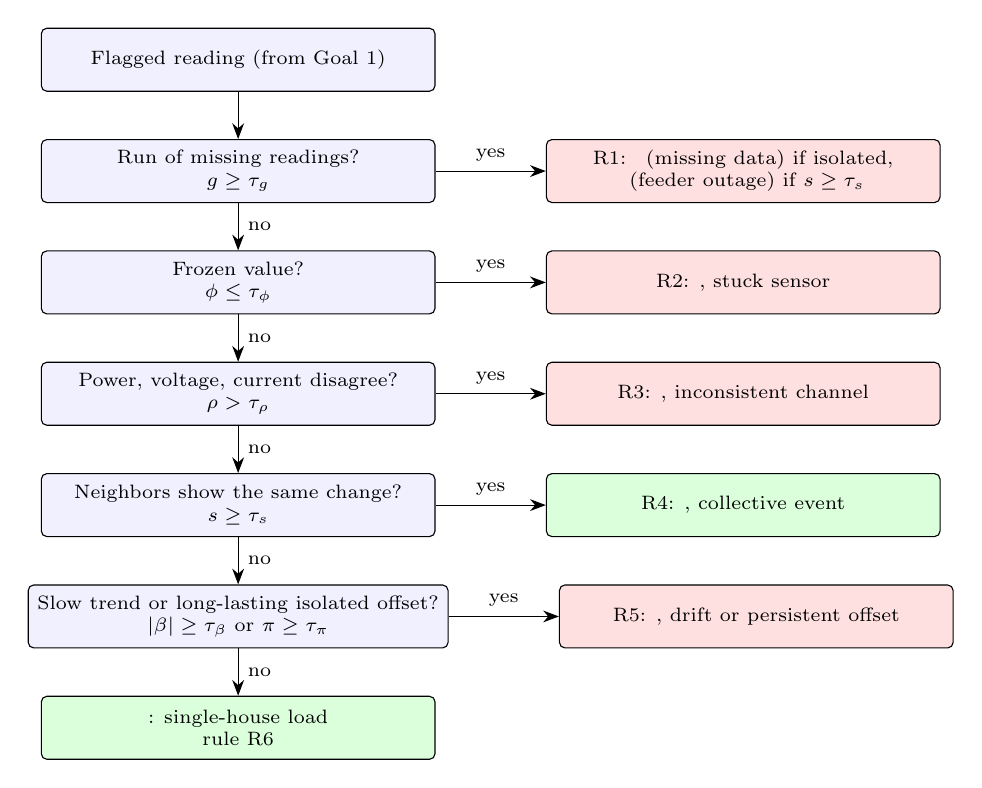
\begin{tikzpicture}[
  node distance=6mm and 14mm,
  q/.style={draw,rounded corners=2pt,fill=blue!6,align=center,minimum width=50mm,minimum height=8mm,font=\scriptsize},
  r/.style={draw,rounded corners=2pt,align=center,minimum width=50mm,minimum height=8mm,font=\scriptsize},
  fault/.style={r,fill=red!12}, event/.style={r,fill=green!14},
  >={Stealth[length=2mm]}, lab/.style={font=\scriptsize,midway,above}]
\node[q] (s0) {Flagged reading (from Goal 1)};
\node[q,below=of s0] (q1) {Run of missing readings?\\ $g\ge\tau_g$};
\node[q,below=of q1] (q2) {Frozen value?\\ $\phi\le\tau_\phi$};
\node[q,below=of q2] (q3) {Power, voltage, current disagree?\\ $\rho>\tau_\rho$};
\node[q,below=of q3] (q4) {Neighbors show the same change?\\ $s\ge\tau_s$};
\node[q,below=of q4] (q5) {Slow trend or long-lasting isolated offset?\\ $|\beta|\ge\tau_\beta$ or $\pi\ge\tau_\pi$};
\node[event,below=of q5] (e2) {\GE{}: single-house load\\ rule R6};
\node[fault,right=of q1] (r1) {R1: \MF{} (missing data) if isolated,\\ \GE{} (feeder outage) if $s\ge\tau_s$};
\node[fault,right=of q2] (r2) {R2: \MF{}, stuck sensor};
\node[fault,right=of q3] (r3) {R3: \MF{}, inconsistent channel};
\node[event,right=of q4] (r4) {R4: \GE{}, collective event};
\node[fault,right=of q5] (r5) {R5: \MF{}, drift or persistent offset};
\draw[->] (s0)--(q1);
\foreach \a/\b in {q1/q2,q2/q3,q3/q4,q4/q5,q5/e2}{\draw[->] (\a)--node[right,font=\scriptsize]{no}(\b);}
\foreach \a/\b in {q1/r1,q2/r2,q3/r3,q4/r4,q5/r5}{\draw[->] (\a)--node[lab]{yes}(\b);}
\end{tikzpicture}
\caption{Rule cascade turning the evidence vector into a verdict. All thresholds $\tau$ are calibrated on the
validation split and stored in a versioned configuration file, not hard-coded.}
\label{fig:rules}
\end{figure}

\begin{table}[H]
\centering
\small
\begin{tabularx}{\textwidth}{@{}>{\raggedright\arraybackslash}p{0.9cm}>{\raggedright\arraybackslash}p{4.2cm}>{\raggedright\arraybackslash}p{3cm}L@{}}
\toprule
\textbf{Rule} & \textbf{Condition} & \textbf{Verdict} & \textbf{Reason sentence (template)} \\
\midrule
R1 & $g\ge\tau_g$ & \MF{} (missing data) if $s<\tau_s$; \GE{} (feeder outage) otherwise & ``\{share\} of this house's readings are missing; \{n\} of \{N\} other houses on the feeder are also affected.'' \\ \\
R2 & $\phi\le\tau_\phi$ for $\ge w$ steps & \MF{} (stuck sensor) & ``The reading has not changed for \{hours\} h; normally it varies by \{x\} kW.'' \\ \\
R3 & $\rho>\tau_\rho$ & \MF{} (channel $k^\ast$) & ``Reported power is \{ratio\}$\times$ what voltage and current imply (limit \{tau\}); channel \{k\} is the odd one out.'' \\ \\
R4 & $s\ge\tau_s$, $\rho\le\tau_\rho$ & \GE{} (collective) & ``\{n\} of \{N\} houses on feeder \{f\} changed together and their electrical readings agree.'' \\ \\
R5 & $s<\tau_s$, and $|\beta|\ge\tau_\beta$ or $\pi\ge\tau_\pi$ & \MF{} (drift or persistent offset) & ``This house has been moving away from its neighbors by \{pct\}\% per day / for \{hours\} h.'' \\ \\
R6 & $s<\tau_s$, $\rho\le\tau_\rho$, short-lived & \GE{} (single-house load) & ``Only this house changed, briefly, and power, voltage and current agree: an appliance switching on is the likely cause.'' \\
\bottomrule
\end{tabularx}
\caption{Rule table}
\label{tab:rules}
\end{table}

The channel $k^\ast$ in R3 is the channel with the largest $|z^{(k)}|$, because a mismatch between power, voltage and current shows that a channel is wrong but not which one.

An isolated reading that is electrically consistent and short-lived (R6) is not called a fault, because a
single house switching on a large appliance is a real event; the neighbors alone cannot tell it apart from
a faulty meter, so consistency and duration are used as well. The same reasoning is why a long-lasting
isolated offset is sent to R5 rather than R6.

\subsection{Confidence Score}
\label{sec:confidence}
The confidence $c_{i,t}\in[0,1]$ is meant to be read as the probability that the reported verdict is
correct. It is built from three inputs, each of which can be inspected on its own:
\begin{enumerate}[leftmargin=*,itemsep=2pt]
  \item the Isolation Forest score $a_{i,t}$, standardized against its distribution on the clean training
        period, $\tilde a_{i,t}$;
  \item the \emph{rule margin} $m_{i,t}\in[0,1]$, which measures how clearly the rule that fired was
      satisfied. Each condition of that rule compares an evidence value $e_j$ with a threshold $\tau_j$.
      For each condition we compute its relative distance from the threshold,
      $\min\{1,\,|e_j-\tau_j|/\tau_j\}$, which is $0$ when the value sits exactly on the threshold and
      $1$ when it is at least one threshold-width away. The margin $m_{i,t}$ is the smallest of these
      values over the conditions of the rule, so a verdict is only as clear as its most borderline
      condition. A reading that barely crosses a threshold therefore gets a small margin.
  \item an \emph{agreement flag} $\kappa_{i,t}\in\{0,1\}$ saying whether an independent statistical check
        also finds the reading abnormal: $|z^{(P)}_{i,t}|$ above a threshold, in the spirit of the explicit
        sigma rule used in rule-aware prompting~\cite{ruleaware}.
\end{enumerate}
The inputs are mapped to a probability with Platt scaling, one of the calibration techniques listed in the trust-calibration literature~\cite{trustcal}, which is a logistic regression with only four coefficients that can be printed and read:
\begin{equation}
  c_{i,t}\;=\;\sigma\!\bigl(\beta_0+\beta_1\tilde a_{i,t}+\beta_2 m_{i,t}+\beta_3\kappa_{i,t}\bigr),
\end{equation}
where $\sigma$ is the logistic function. 

The coefficients are fitted on events whose true label is known from the injection log, with ``the verdict was correct'' as the target. If the resulting calibration curve is poor, isotonic regression, another technique from the same  iterature~\cite{trustcal}, is the alternative.

We do not assume that the result is calibrated; we measure it (Section~\ref{sec:evaluation}). This matters because the confidence-based routing of Goal~3 assumes reasonably calibrated confidence: an overconfident model may delegate dangerous decisions to the AI, and an underconfident one may defer everything to humans~\cite{trustcal}.

\paragraph{Data used for fitting.} The training portion of the dataset is kept free of injected anomalies and is used only for
the baselines $\mu,\sigma$ and the standardization of $a$. The validation and test periods contain injected
faults and events with known labels. The validation period is split by episode into two parts: the first
fits the thresholds $\tau$, the second fits the coefficients $\beta$. The test period is touched only for the
final report. Splitting by episode rather than by row keeps near-duplicate neighboring readings from leaking
between sets.

\subsection{From Evidence to Plain Language}
\label{sec:language}
Figure~\ref{fig:pipeline} shows how the verdict and the evidence become the text that the operator reads,
following the chain model $\rightarrow$ SHAP $\rightarrow$ evidence $\rightarrow$ RAG $\rightarrow$ LLM text.
Full explanations are generated only for flagged events, never for every normal reading, to keep latency and
cost down.

\begin{figure}[htbp]
\centering
\resizebox{\textwidth}{!}{%
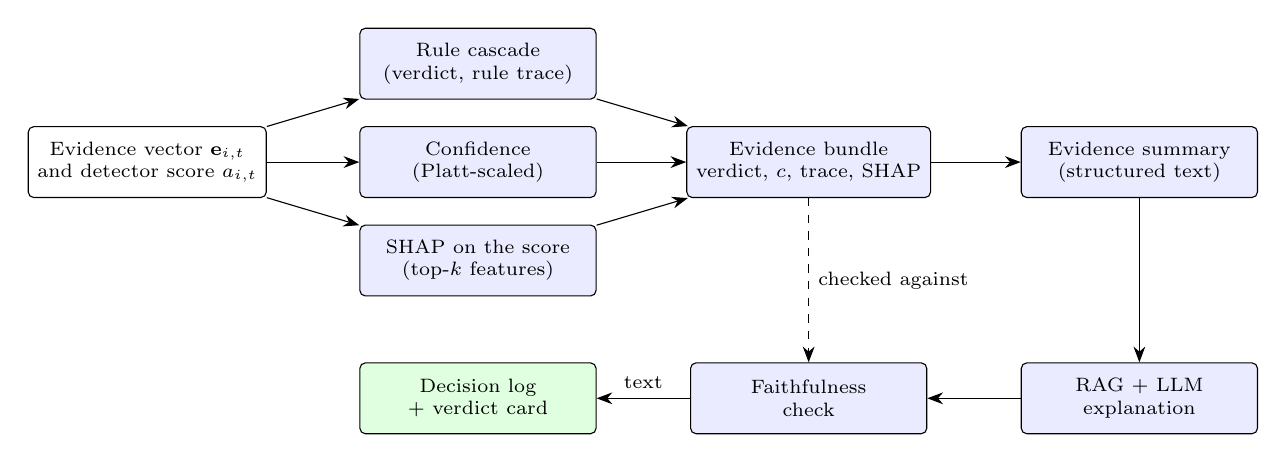
\begin{tikzpicture}[
  b/.style={draw,rounded corners=2pt,align=center,minimum width=30mm,minimum height=9mm,font=\scriptsize},
  core/.style={b,fill=blue!8}, result/.style={b,fill=green!12},
  >={Stealth[length=2mm]}]
\node[b] (ev) at (0,0) {Evidence vector $\mathbf{e}_{i,t}$\\ and detector score $a_{i,t}$};
\node[core] (rules) at (4.2,1.25) {Rule cascade\\ (verdict, rule trace)};
\node[core] (cal) at (4.2,0) {Confidence\\ (Platt-scaled)};
\node[core] (shap) at (4.2,-1.25) {SHAP on the score\\ (top-$k$ features)};
\node[core] (bundle) at (8.4,0) {Evidence bundle\\ verdict, $c$, trace, SHAP};
\node[core] (tpl) at (12.6,0) {Evidence summary\\ (structured text)};
\node[core] (llm) at (12.6,-3.0) {RAG + LLM\\ explanation};
\node[core] (val) at (8.4,-3.0) {Faithfulness\\ check};
\node[result] (log) at (4.2,-3.0) {Decision log\\ + verdict card};
\draw[->] (ev)--(rules); \draw[->] (ev)--(cal); \draw[->] (ev)--(shap);
\draw[->] (rules)--(bundle); \draw[->] (cal)--(bundle); \draw[->] (shap)--(bundle);
\draw[->] (bundle)--(tpl);
\draw[->] (tpl)--(llm);
\draw[->] (llm)--(val);
\draw[->,dashed] (bundle)--node[right,font=\scriptsize]{checked against}(val);
\draw[->] (val)--node[above,font=\scriptsize]{text}(log);
\end{tikzpicture}}
\caption{Explanation pipeline}
\label{fig:pipeline}
\end{figure}

The language model only receives the evidence bundle and retrieved snippets and writes about them; the faithfulness check compares its text with the same bundle. If the check rejects the text, the evidence summary is logged and shown instead.

\subsubsection*{Step 1: attributions with SHAP}
The rules say what kind of problem it is; SHAP says why the detector flagged the reading in the first
place. SHAP assigns each input feature a value showing how much it pushed the detector's score for this
reading up or down relative to a baseline, and it is model-agnostic. We apply the \texttt{shap} library to the
Isolation Forest of Goal~1, on its rolling features, and only on flagged events. If a second detector (the
autoencoder stretch goal of Goal~1) is added, SHAP applies to it in the same way. Each feature is tied to a
sentence template by a small lexicon, which is how a number becomes a statement
(Table~\ref{tab:lexicon}).

\begin{table}[H]
\centering
\small
\begin{tabularx}{\textwidth}{@{}>{\raggedright\arraybackslash}p{3.2cm}L@{}}
\toprule
\textbf{Feature} & \textbf{Sentence template} \\
\midrule
$z$-score & ``Power is \{z\} standard deviations \{above/below\} this house's usual level for \{hour\}.'' \\ \\
Rolling mean & ``Average power over the last \{w\} steps is \{x\} kW against a usual \{y\} kW.'' \\ \\
Rolling standard deviation & ``The reading has varied by only \{x\} kW over the last \{hours\} h; normally \{y\} kW.'' \\ \\
Rate of change & ``Power changed by \{x\} kW in one step; the usual maximum change is \{y\} kW.'' \\ \\
Hour of day / day of week & ``This level is unusual for \{hour\} on a \{day\}.'' \\
\bottomrule
\end{tabularx}
\caption{Excerpt of the feature lexicon that turns attributions into sentences (one entry per detector
feature; the evidence quantities of Table~\ref{tab:evidence} have their own sentences in Table~\ref{tab:rules}).}
\label{tab:lexicon}
\end{table}

\subsubsection*{Step 2: structured evidence summary}
A deterministic step assembles the evidence bundle into a summary: a headline (verdict, channel and
confidence), the strongest reasons (the rule's reason sentence first, then the highest SHAP contributions),
a \emph{what would change this verdict} line generated from the rule thresholds, and a suggested check. This
follows the recommendation, in a review of AI approaches for smart-grid reliability, to combine local feature
attribution, counterfactuals and logged explanations~\cite{review2025}. The summary is the input of the
language model and also the text shown if the faithfulness check fails. An illustrative card (values invented
for illustration, not experimental results):

\begin{lstlisting}
Event E-000142 | House H17 (feeder F2) | 2025-03-14 19:30
VERDICT: METER FAULT, power channel          CONFIDENCE: 0.91

Why:
 1. Reported power is 8.7x what voltage and current imply
    (limit 1.05x) -> rule R3.
 2. Isolated: 0 of 9 other houses on feeder F2 show a change
    (a real event needs at least 3 of 9).
 3. Power is 7.9 standard deviations above this house's usual level for 19:30; voltage and current are normal.
 
This would be a GENUINE EVENT instead if: >= 3 neighbors showed the same change, 
or the power/voltage/current mismatch fell below 5%.

Suggested check: compare the meter register with a handheld reading; inspect the power channel.
\end{lstlisting}

\subsubsection*{Step 3: RAG and LLM explanation with a faithfulness check}
The language model turns the evidence summary into a readable diagnosis and can add context that a
template cannot, such as earlier incidents at the same house. It receives the evidence bundle as structured
data together with a few retrieved snippets from a small corpus: descriptions of the fault kinds, the
anomaly taxonomy and earlier log entries for the same house. It is asked to justify the verdict against an
explicit, stated rule, as in rule-aware prompting for grid telemetry~\cite{ruleaware}, and it may not alter
the verdict or the confidence.

Before the text is displayed, a faithfulness check compares it with the evidence bundle:
\begin{itemize}[leftmargin=*,itemsep=1pt]
  \item every reason it names must be a fired rule or one of the top-$k$ SHAP features;
  \item every number it quotes must match the logged value up to rounding;
  \item the verdict and the confidence must be those in the log.
\end{itemize}
If any test fails, the evidence summary is shown instead and the event is logged with that fact. The check
is needed because a study of retrieval-augmented LLM post-processing for anomaly detection found only a
modest gain from the language model, and explanation faithfulness did not improve with retrieval~\cite{ragaudit}.
We therefore treat the LLM as a layer that describes the evidence, not as a source of reasoning.

\subsection{Auditable Decision Log}
\label{sec:log}
Every flagged event produces one record in an append-only JSON Lines file. The record is grouped around the
three questions the challenge asks (Table~\ref{tab:log}); an abridged example follows. Other components, such
as the escalation logic of Goal~3, append their own fields (governance decision, human decision, final
outcome) to the same record; this section defines only the fields produced by detection, conclusion and
explanation.

\begin{table}[H]
\centering
\small
\begin{tabularx}{\textwidth}{@{}>{\raggedright\arraybackslash}p{2.8cm}L@{}}
\toprule
\textbf{Block} & \textbf{Fields} \\
\midrule
\texttt{detected} & event id, timestamp, house id, detected anomaly, model and version, anomaly score \\ \\
\texttt{concluded} & verdict, sub-type, suspect channel, confidence $c$, agreement flag \\ \\
\texttt{why} & rule trace (rule id, measured value, threshold, passed or not), SHAP evidence, neighborhood support, retrieved sources \\ \\
\texttt{explanation} & LLM diagnosis, result of the faithfulness check, text actually shown \\
\bottomrule
\end{tabularx}
\caption{Structure of a decision log record.}
\label{tab:log}
\end{table}

\begin{lstlisting}
{"event_id":"E-000142","ts":"2025-03-14T19:30:00","house":"H17","feeder":"F2",
 "detected":{"model":"isolation-forest-v1","score":0.82,"flag":true},
 "concluded":{"verdict":"METER_FAULT","subtype":"inconsistent_channel",
   "channel":"power_kw","confidence":0.91,"agreement":true},
 "why":{"rules":[{"id":"R3","measured":8.7,"threshold":1.05,"passed":true},
                 {"id":"R4","measured":0.0,"threshold":0.33,"passed":false}],
        "shap":[["z_score",0.41],["rolling_mean",0.33],["rate_of_change",0.12]],
        "neighbors":"0/9","sources":["fault_kinds#freeze","incident#E-000097"]},
 "explanation":{"llm_diagnosis":"...","faithfulness":"pass","shown":"llm"}}
\end{lstlisting}
(The values are invented for illustration.) The record keeps the exact inputs and the version of the
thresholds and models, so a verdict can be reproduced and reviewed later.

\subsection{How We Will Evaluate Explanations and Confidence}
\label{sec:evaluation}
The injection log of the dataset records the true kind, channel, scope and timing of every injected event,
which allows verdicts and explanations to be tested against ground truth rather than only judged by eye.
Genuine anomalies are rare compared with normal readings, so plain accuracy is not reported; we use
precision, recall, F1 and false-positive rate.

\begin{table}[H]
\centering
\small
\begin{tabularx}{\textwidth}{@{}>{\raggedright\arraybackslash}p{3.1cm}LL@{}}
\toprule
\textbf{Aspect} & \textbf{Measure} & \textbf{Method} \\
\midrule
Confidence quality & Calibration curve and Brier score~\cite{trustcalpage}; verdict accuracy within confidence bands & Test period, per class and overall \\ \\
Verdict correctness & Precision, recall, F1 and false-positive rate per class, with episode counts & Compare with the injection log, on the normal and on the subtle severity set \\ \\
Explanation correctness & Share of faults whose named channel equals the injected channel; share whose scope (collective or isolated) is right & Injection log versus the \texttt{why} block \\ \\
LLM faithfulness & Share of LLM texts accepted by the faithfulness check; kinds of statements rejected & Automatic check on all flagged events \\ \\
Does the LLM help & LLM text versus the plain evidence summary, rated on clarity and correctness (1--5) by several team members who do not know which is which & Sample of flagged test events \\ \\
Response latency & Median and 95th-percentile time of rules, SHAP and LLM per flagged event & Timer on the test set \\
\bottomrule
\end{tabularx}
\caption{Evaluation plan for confidence scores and explanations.}
\label{tab:evalplan}
\end{table}

\subsection{Risks and Limitations}
\label{sec:risks}
\begin{itemize}[leftmargin=*,itemsep=2pt]
  \item \textbf{Derived electrical channels.} If voltage, current and power factor are
        derived from consumption in the neighborhood dataset, the consistency check $\rho$ is easy by
        construction, and its value on real meters would be lower. In that case we add measurement noise
        before testing, state this limit in the report, and need the injector to corrupt individual channels
        for R3 to be meaningful.
  \item \textbf{Thresholds fitted on injected data.} Thresholds and calibration coefficients are fitted on
        simulated anomalies and may be optimistic. We report results on the subtle severity set as well and
        state this limit explicitly.
  \item \textbf{Correlated features.} SHAP can spread credit among correlated features. The rule trace is
        therefore the primary explanation and SHAP the supporting one.
  \item \textbf{Cost of SHAP.} SHAP is run only on flagged events and its latency is measured; the rule
        trace remains available if it is too slow.
  \item \textbf{Calibration can drift} across seasons or houses; the calibration curve is checked again on
        later events.
  \item \textbf{Convincing but wrong.} A fluent explanation can raise trust beyond what the evidence
        justifies, so every card shows the confidence and the counterfactual line.
  \item \textbf{Language model errors.} The faithfulness check and the fallback to the evidence summary
        limit this, and the acceptance rate of the check is reported.
\end{itemize}

% ===================== END GOAL 2 SECTION =======================

\begin{thebibliography}{99}
\bibitem{ruleaware} ``A Rule-Aware Prompt Framework for Structured Numeric Reasoning in Smart Grids,'' arXiv:2512.12794.
\bibitem{ragaudit} ``Component-Level Contributions of Retrieval-Augmented LLM Post-Processing in Streaming Anomaly Detection,'' \emph{Sensors}, 2026.
\bibitem{trustcal} ``Confidence-Based Trust Calibration in Human-AI Teams,'' SAI, vol.~16, no.~12.
\bibitem{trustcalpage} ``Trust Calibration in AI,'' Emergent Mind overview page, \url{https://www.emergentmind.com/topics/trust-calibration-in-ai}.
\bibitem{review2025} ``Comprehensive review of AI-driven approaches for smart grid stability and reliability,'' ScienceDirect, 2025.
\bibitem{timefreq} ``Time and Frequency Domain-based Anomaly Detection in Smart Meter Data,'' arXiv:2504.18231.
\bibitem{multiuser} ``Multi-User Energy Consumption Monitoring and Anomaly Detection with Partial Context Information.''
\end{thebibliography}
\end{document}